\noindent

\includegraphics[height=1.25cm]{images/pictograms/benchmark}

\includegraphics[height=1.25cm]{images/pictograms/under_construction}

\includegraphics[height=1.25cm]{images/pictograms/FEM}

\includegraphics[height=1.25cm]{images/pictograms/paraview}

%%%%%%%%%%%%%%%%%%%%%%%%%%%%%%%%%%%%%%%%%%%%%%%%%%%%%%%%%%%%%%%%%%%%%%%%%%%%%%%%%%%%%%%%%%%%%%%%%%%

\begin{flushright} {\tiny {\color{gray} python\_codes/fieldstone\_133/text.tex}} \end{flushright}

%\lstinputlisting[language=bash,basicstyle=\small]{python_codes/template_keywords.key}

\par\noindent\rule{\textwidth}{0.4pt}

\begin{center}
\inpython
{\small Code: \url{https://github.com/cedrict/fieldstone/tree/master/python_codes/fieldstone_133}}
\end{center}

\par\noindent\rule{\textwidth}{0.4pt}
%%%%%%%%%%%%%%%%%%%%%%%%%%%%%%%%%%%%%%%%%%%%%%%%%%%%%%%%%%%%%%%%%%%%%%%%%%%%%%%%%%%%%%%%%%%%

The benchmark is described fully in Section~\ref{MMM-ss:anconv}. 
The following results have been obtained with $k=4$.
Taylor-Hood $Q_2\times Q_1$ elements are used with an isoparametric mapping. 
This \stone is based on \stone~21 (please refer to this one first 
before reading any further).

The idea here is to test the Double Jacobian algorithm presented in \textcite{moth20} (2020)
as thoroughly described and worked out in Section~\ref{MMM-ss:doublejac}.

In the code this can be toggled on/off by means of the {\python DJ} boolean.
Also, the internal numbering of nodes has been completely reworked with regards to 
the one used in \stone~21 to match with the theory.

The node layout is as follows:

\begin{center}
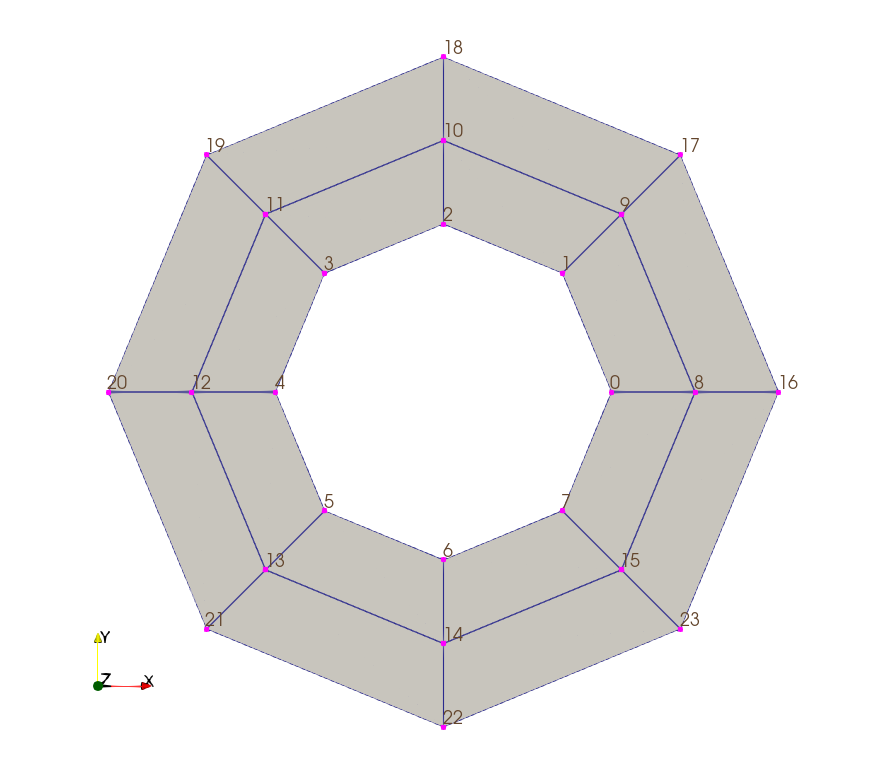
\includegraphics[width=8cm]{python_codes/fieldstone_133/images/nodes}
\end{center}
with
\begin{verbatim}
nelr= 1
nelt= 4
nel= 4
NfemV= 48
NfemP= 8
0 | [ 0 16 18  2  8 17 10  1  9]
1 | [ 2 18 20  4 10 19 12  3 11]
2 | [ 4 20 22  6 12 21 14  5 13]
3 | [ 6 22 16  0 14 23  8  7 15]
\end{verbatim}








